\chapter{Patched MPO-MPO Contractions}
\label{chap:MPOcontr}
MPO-MPO contractions are widely recognized as a critical computational bottleneck in tensor-network algorithms, appearing frequently in applications like real-time evolution \cite{Paeckel2019}, finite-temperature simulations \cite{Verstraete2004}, two-particle field theory calculations \cite{Rohshap2025} and standard ground-state DMRG computations \cite{Schollwock2011}. Even when employing optimal contraction strategies, the computational complexity typically scales unfavorably with increasing bond dimensions rapidly becoming the dominant cost for large-scale calculations \cite{Schollwock2011,Rohshap2025,Paeckel2019}.

(Q)TCI makes it possible to encode intricate functions in a highly compact tensor‐train form, greatly facilitating the numerical evaluation of otherwise challenging integrals \cite{Fernandez2022,Fernandez2024,Rohshap2025}.  
Besides the favourable complexity of the TCI algorithm itself, in general tensor representations are especially beneficial for convolution–type integrals, e.g.\ $h(x,y)\;=\;\int_{0}^{1}\! \mathrm{d}t\,f(x,t)\,g(t,y),$
because they allow such integral to be carried out by simply contracting the MPOs representing the two integrands. More importantly, the contraction yields a ready‐made, reusable tensor‐train representation of the result~\(h\).

While (Q)TCI substantially mitigates the cost of setting up convolution–type integrals, the subsequent MPO–MPO contraction still scales steeply with the bond dimensions of the two factors--typically $\order(\chi^{4})$ \cite{Stoudenmire2010}-- depending on the algorithm employed.  This rank dependence motivates \emph{distributing} the contraction across smaller sub-problems whose bond dimensions are capped, in the spirit of
patched (Q)TCI.  We refer to such strategies collectively as \emph{patched MPO–MPO contractions}.

The remainder of this chapter is organised as follows: \prettyref{sec:MPOMPOcontr} reviews conventional MPO–MPO contraction schemes and establishes the notation used later;  \prettyref{sec:PatchMPOMPOContr} introduces the patched approach, analysing its advantages and resource scaling for several representative tensor products; finally, \prettyref{sec:AdaptivePatchMPOMPOContr} presents a new \emph{adaptive} contraction algorithm that, analogously to pQTCI, dynamically partitions the tensors and caps the local bond dimension, thereby balancing the contraction workload across patches.

\section{MPO-MPO Contractions: standard algorithms}
\label{sec:MPOMPOcontr}
A variety of well–established algorithms can contract two MPOs with high efficiency.  
Before reviewing these methods, we introduce the notation and conventions commonly adopted in the tensor-network literature, beginning with the central object of interest: the \textit{Matrix Product Operator} (\textit{MPO}).
\subsection{Matrix Product Operators}
Consider the tensor-train representation
\begin{equation}
    \widetilde{M}_{\bsigma\bsigma'} = \raisebox{-5.5mm}{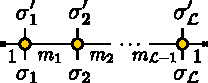
\includegraphics{figures/GenericMPO.pdf}}, \quad \text{with} \quad  M_\ell = \raisebox{-5.5mm}{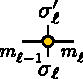
\includegraphics{figures/MPOSiteTensor.pdf}}.
\end{equation}
In the quantum-many-body community such a tensor train  with two physical legs per site is known as a \textit{Matrix Product Operator} (\textit{MPO}) \cite{Hubig2017, McCulloch2008, vonDelftTNNotes, Schollwock2011}. In numerical mathematics the same object appears under the name \textit{Tensor-Train Operator} (\textit{TTO}) \cite{Oseledets2011}. Each four-legged core $M_\ell$ carries two virtual indices and two physical indices, and the largest virtual dimension, $\chi = \max_\ell m_\ell$, is called the rank of the MPO, mirroring the definition for matrix-product states (MPSs). MPOs are routinely built to encode operators—Hamiltonians, density matrices, transfer matrices, projectors—that act on an MPS \cite{Hubig2017, Verstraete2008}. They underpin modern DMRG algorithms, time-evolution schemes, finite-temperature purification, and many other tensor-network techniques. 

The emergence of cross–approximation techniques has extended the relevance of MPOs to high–dimensional quadrature and convolution problems. A key property is that \emph{any} matrix-product state (MPS) can be recast as an MPO simply by fusing pairs (or groups) of physical indices. For an MPS comprising \(2\mathcal{L}\)
sites, the transformation is schematically
\begin{equation}
    \raisebox{-1.5cm}{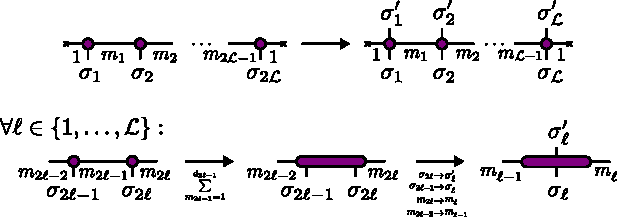
\includegraphics{figures/MPStoMPO.pdf}}
    \label{eq:MPStoMPO}
\end{equation}
where consecutive physical indices \((\sigma_{2\ell-1},\sigma_{2\ell})\) are merged into a single input–output pair
\(\bigl(\sigma_{2\ell-1},\sigma_{2\ell}\bigr)\equiv
 (\sigma'_{\ell},\sigma_{\ell})\).
This simple regrouping turns the state into an operator, enabling the same compressed representation to serve both as a multidimensional function and as an MPO contraction kernel.
For a generic MPS, one simply fuses multiple neighbouring indices—for example $\sigma_\ell,\sigma_{\ell+1},\sigma_{\ell+2} \to  \left((\sigma_\ell,\sigma_{\ell+1}),\sigma_{\ell+2}\right):=(\sigma_\ell,\sigma'_\ell)$—to obtain the desired operator form.

Given two matrix-product operators (MPOs)
\begin{equation}
    \widetilde{A}_{\bsigma\bsigma'} = \raisebox{-5.5mm}{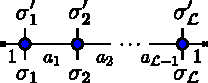
\includegraphics{figures/AMPO.pdf}}, \qquad \widetilde{B}_{\bsigma'\bsigma''} = \raisebox{-7mm}{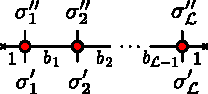
\includegraphics{figures/BMPO.pdf}}
    \label{eq:2MPOs}
\end{equation}
our goal is to form their product $\sum_{\bsigma'} \widetilde{A}_{\bsigma\bsigma'} \widetilde{B}_{\bsigma'\bsigma''}$:
\begin{equation}
    \raisebox{-8mm}{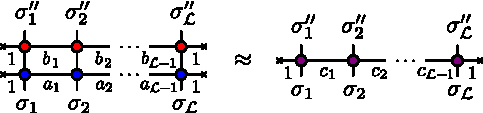
\includegraphics{figures/MPOMPOcontr.pdf}} := \widetilde{C}_{\bsigma\bsigma''}.
\end{equation}
If $\widetilde{A}$ and $\widetilde{B}$ both have rank $\chi$ we want the final result $\widetilde{C}$ also to have rank $\simeq \chi$. Several contraction strategies exist. Below we outline the familiar \textit{zip-up} algorithm for completeness of this manuscript; alternative schemes available in modern tensor-network toolkits include the \textit{fitting} routine of Stoudenmire and White \cite{Stoudenmire2010} and the \textit{density-matrix} algorithm described in the tensornetwork.org documentation \cite{tensornetwork.org}.
\subsection{The zip-up algorithm}
Consider two MPOs of identical bond dimensions~\(\chi\) (cf. \prettyref{eq:2MPOs}) and phyiscal dimensions $d$. 
\begin{figure}[ht!]
    \centering
    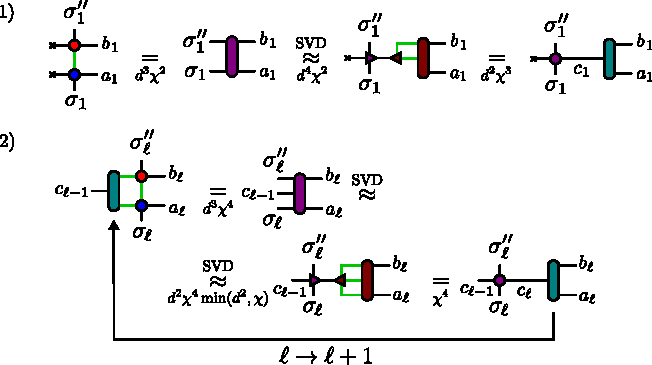
\includegraphics{figures/ZipUp.pdf}
    \caption{The zip-up MPO-MPO contraction algorithm. Each step is labelled with its computational cost. At each iteration the indices coloured green indicate the next contraction to be performed. Refer to the main manuscript for additional details.}
    \label{fig:zipupalg}
\end{figure}

\prettyref{fig:zipupalg} sketches the \emph{zip-up} algorithm, an efficient left-to-right MPO contraction procedure:
\begingroup
\renewcommand{\labelenumi}{(\arabic{enumi})}
\begin{enumerate}
\item Begin at the leftmost site.  
  Contract the shared physical index \(\sigma'_{1}\) of the two site tensors to form a four-legged object.  
  Treat \(\bigl(\sigma_{1},\sigma''_{1}\bigr)\) as the row index
  and \(\bigl(a_{1},b_{1}\bigr)\) as the column index of a matrix, then apply an SVD.  
  The resulting left isometry
  \(\raisebox{-0.1mm}{
\includegraphics{figures/LeftIsometry.pdf}}\) becomes the first core of the product MPO, while the residual
  (the diagonal and right singular tensors) is contracted into a single “left-over” tensor.
  Truncate the SVD either by setting a maximum rank or by discarding singular values below a local tolerance $\tau_{\text{loc}}$.

\item Move one site to the right.  
  Contract the left-over tensor with two new site tensors out of the factor MPOs, fuse the indices
  \(\bigl(\sigma_{\ell},c_{\ell-1},\sigma''_{\ell}\bigr)\) and
  \(\bigl(a_{\ell},b_{\ell}\bigr)\) into the new row/column pair and repeat the SVD and truncation as in step~(1).

\end{enumerate}
\endgroup
 After each SVD step the row index of the singular value matrix will constitute the new bond dimension $c_\ell$ for the product MPO. The zip-up procedures scales as \begin{equation}
    \order(\chi^4d^4\mL)
\end{equation}
with the parameters of our input MPOs.  

A well–known drawback of the zip-up scheme is that the global approximation error of the resulting MPO is not rigorously bounded by the local SVD tolerances \(\varepsilon_{\text{loc}}\) \cite{Stoudenmire2010}.  In practice, however, tightening \(\varepsilon_{\text{loc}}\) usually reduces the overall
error.  Several best-practice remedies are commonly employed:

\begin{itemize}
  \item \emph{Right–canonical preconditioning.}  
        Transform both the two input MPOs to right-canonical form
        \cite{vonDelftTNNotes}.  This stabilises the local factorizations and mitigates ill-conditioning.
  \item \emph{Error-based truncation.}  
        Instead of imposing a hard rank cap $\chi$, truncate each SVD by discarding singular values whose squared weight falls below a prescribed cutoff, thereby adapting the rank to the local spectrum.
  \item \emph{Hybrid refinement.}  
        Perform an initial left-to-right zip-up sweep with a fixed rank $\chi$ to obtain a rough product MPO, then feed this guess into the \emph{fitting} algorithm of Ref. \cite{Stoudenmire2010}, which iteratively refines the bond dimensions while monitoring the global error.
\end{itemize}

These strategies balance accuracy and efficiency, providing tighter control over the final approximation error without incurring prohibitive cost. Adopting an error-based type of truncation, while monitoring the local bond dimensions of the resulting MPO, will allow us to use the zip-up routine for our patched version of MPO contraction algorithms.

\section{Patched MPO-MPO Contractions}
\label{sec:PatchMPOMPOContr}

MPO–MPO contractions rank among the most demanding kernels in tensor–network computations: their arithmetic cost scales roughly as the \(\chi^{4}\) power of the bond dimension \(\chi\) of the two input operators.  Such a steep dependence quickly turns the contraction step into a major bottleneck.  
Because the bond dimension is the dominant cost driver, a \emph{distributed} strategy that caps the \emph{local} bond dimension—mirroring the philosophy of patched QTCI—promises substantial savings.

In what follows we introduce this strategy, which we call
\emph{patched MPO–MPO contraction}, and show how it can already accelerate several representative tensor contractions encountered in practical applications. We start by defining \textit{patched MPOs} and by illustrating how to contract them.

\subsection{Patched contraction logic}
The output produced by pQTCI contains objects with the schematic form

\begin{equation}
    \raisebox{-7mm}{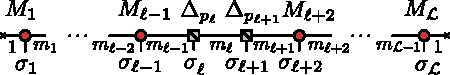
\includegraphics{figures/MultplePatchMPS.pdf}}.
    \label{eq:patchedMPS}
\end{equation}

Suppose we promote this patched MPS to an MPO so that it can enter some contraction procedure. The local MPS-to-MPO mapping depends on the site index~$\ell$, hence on the way the MPS cores are grouped; from \prettyref{eq:MPStoMPO} one obtains
\begin{align}
    \label{eq:patchMPStoMPO}
        \nonumber &\raisebox{-0.6cm}{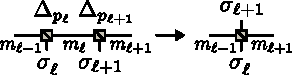
\includegraphics{figures/patchMPStopatchMPO_SiteTensor.pdf}} &=&\quad \begin{cases}
		[\mathds{1}]_{m_{\ell-1},m_{\ell+1}} & \text{if } \sigma_\ell = p_\ell \wedge \sigma_{\ell +1} = p_{\ell +1}\\
		[0]_{m_{\ell-1},m_{\ell+1}} & \text{otherwise},
        \end{cases}\\[6pt]
        &\raisebox{-0.6cm}{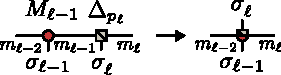
\includegraphics{figures/patchMPStoBottomHalfPatchMPO.pdf}} &=&\quad \begin{cases}
		[M^{\sigma_{\ell-1}}]_{m_{\ell-2},m_{\ell}} & \text{if }\sigma_\ell = p_\ell\\
		[0]_{m_{\ell-2},m_{\ell}} & \text{otherwise},
        \end{cases}\\[6pt]
        \nonumber &\raisebox{-0.6cm}{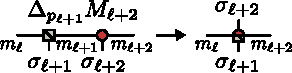
\includegraphics{figures/patchMPStoTopHalfPatchMPO.pdf}} &=& \quad \begin{cases}
		[M^{\sigma_{\ell+2}}]_{m_{\ell},m_{\ell+2}} & \text{if } \sigma_{\ell+1} = p_{\ell+1} \\
		[0]_{m_{\ell},m_{\ell+2}} & \text{otherwise}.
        \end{cases}  
\end{align}

Whenever we are contracting two patched MPOs, which may be folded from MPSs of the type in \prettyref{eq:patchedMPS}, the product is non--the vanishing only if for those sites on which both internal indices are projected, say $\sigma_\ell^{\prime A} = p_\ell^{\prime A}$ and $\sigma_\ell^{\prime B} = p_\ell^{\prime B}$, they are projected to the same value, i.e. if $p_\ell^{\prime A} = p_\ell^{\prime B}$. Consider the following patched MPOs
\begin{equation}
    \label{eq:patchMPOs}
    \begin{aligned}
        \widetilde{B}^{p''_3,p''_4}_{\bsigma'\bsigma''} &= \raisebox{-7mm}{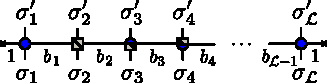
\includegraphics{figures/BProjMPO.pdf}}.\\
        \widetilde{A}^{p_2,p'_2,p_3,p'_4}_{\bsigma\bsigma'} &= \raisebox{-5.5mm}{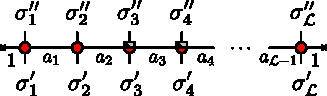
\includegraphics{figures/AProjMPO.pdf}} 
    \end{aligned}  
\end{equation}
They always yield a result of the form

\begin{equation}
    \label{eq:resultPatchContr}
        \widetilde{C}^{p_2,p_3,p''_3,p''_4}_{\bsigma\bsigma''} = \raisebox{-7mm}{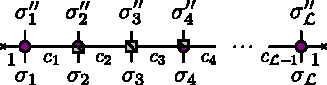
\includegraphics{figures/CProjMPO.pdf}}.
\end{equation}
when contracting over the shared indices $\bsigma'$.
By contrast, two MPOs shaped as
\begin{equation}
    \label{eq:patchMPOsMaybe}
    \begin{aligned}
      \widetilde{B}^{p'_2,p'_3,p''_3}_{\bsigma'\bsigma''}  &= \raisebox{-7mm}{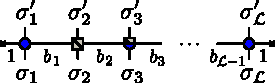
\includegraphics{figures/BProjMPO_vanish.pdf}}\\
         \widetilde{A}^{p_2,p'_2,p'_3}_{\bsigma\bsigma'} &= \raisebox{-5.5mm}{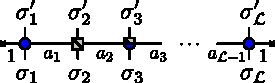
\includegraphics{figures/AProjMPO_vanish.pdf}}
    \end{aligned}  
\end{equation}
produce a non--zero contraction only when the projected internal indices match, \textit{i.e.} $p'^{A}_{2}=p'^{B}_{2}$ and $p'^{A}_{3}=p'^{B}_{3}$.  In other words, to obtain a non--vanishing outcome, any internal index that is projected must be projected onto the \emph{same} value in both factors; the external indices ($\bsigma,\bsigma''$ in \prettyref{eq:patchMPOs}) place no such restriction. All the tensors in \prettyref{eq:patchMPOs}, \prettyref{eq:resultPatchContr} and \prettyref{eq:patchMPOsMaybe} will be hereafter referred to as \textit{patched MPOs} or \textit{patch MPOs}.

Assume that two tensors \(A_{\boldsymbol{\sigma}}\) and
\(B_{\boldsymbol{\sigma}}\) have been decomposed through p(Q)TCI into collections of
patches,
\begin{equation}
    \label{eq:patchCollectionsContr}
  A_{\bsigma}
    \;\approx\;
    \sum_{\widetilde{A}^{(i)}\in\texttt{results}_{A}}\,
        \widetilde{A}^{(i)},
  \qquad
  B_{\boldsymbol{\sigma}}
    \;\approx\;
    \sum_{\widetilde{B}^{(j)}\in\texttt{results}_{B}}\,
        \widetilde{B}^{(j)}.
\end{equation}
After promoting each patch to MPO form (cf. \prettyref{eq:patchMPStoMPO}), the full contraction \(C_{\bsigma,\bsigma''} = \sum_{\bsigma'}A_{\bsigma,\bsigma'}B_{\bsigma'\bsigma''}\) can be assembled patch-wise:
contract every patch \(\widetilde{A}^{(i)}\) with each \emph{compatible} patch \(\widetilde{B}^{(j)}\) (i.e.\ those whose projected internal indices match).  This yields a family of subtensors \(\{\widetilde{C}^{(k)}\}\) which, upon MPO-to-MPS unfolding (cf.\ \prettyref{eq:resultMPSPatchContr}), collectively approximate the target tensor \(C_{\bsigma}\) (unfolding of $C_{\bsigma,\bsigma''}$). In other words, each TT of $\texttt{results}_{A}$ will be contracted with every TT in $\texttt{results}_{B}$ and depending on the compatibility of the projection result in a TT $\widetilde{C}^{(k)}$ part of the patched representation of \(C_{\bsigma}\). The subsequent section will help us clarify this concept with a graphical representation of the \textit{patched contraction} for quantics tensor trains.

\subsection{2D representation of patched contractions}
The product MPO in \prettyref{eq:resultPatchContr} can be unfolded back into a patched MPS by inverting the mapping of \prettyref{eq:MPStoMPO}. To do so, one may perform an SVD or a CI/prrLU on each MPO site tensor or simply read off the local cores from \prettyref{eq:patchMPStoMPO}, in the case of a patched MPO. The resulting MPS reads
\begin{align}
    \label{eq:resultMPSPatchContr}
     \nonumber \widetilde{C}^{p_2,p_3,p''_3,p''_4}_{\bsigma} &= \raisebox{-6mm}{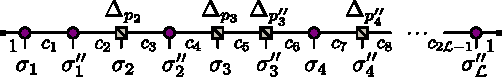
\includegraphics{figures/PatchMPS_ResultContr.pdf}}\\
     {}\\[-5pt]
    \nonumber \widetilde{C}^{p_3,p_5,p_6,p_8}_{\bsigma} &= \raisebox{-6mm}{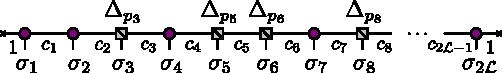
\includegraphics{figures/PatchMPS_ResultContrReshaped.pdf}},
\end{align}
where the second equality is obtained after relabelling site indices and bond dimensions.
The auxiliary cores $\Delta{p_{\ell}}$ encode the subtensor corresponding to the external (non--contracted) indices of $\widetilde{A}$ and $\widetilde{B}$, \textit{i.e.} external (non-contracted) projected indices in $\widetilde{A}$ and $\widetilde{B}$ will be projected indices in $\widetilde{C}$. 

The tensor‐trains in \prettyref{eq:resultMPSPatchContr} closely mirror the TT form of an individual patch produced by the pQTCI algorithm. If each TT physical index has dimension $d_\ell = 2$ we can assume to be working with a two–dimensional, interleaved quantics representation of some function, where each such MPS corresponds to a distinct sub-region of a 2D domain, uniquely labelled by its prefix indices. A full set of these patches can tile the entire domain of the function.

This insight suggests a convenient two-dimensional diagrammatic view of patched contractions. Let us introduce three quantics variables on the unit interval, each resolved with $\mR$ binary digits,
\begin{equation}
    \begin{aligned}
        &x \mapsto x(\bsigma) = \sum_{r=1}^{\mR} \sigma_r 2^{-r} \quad &y \mapsto y(\bsigma'') = \sum_{r=1}^{\mR} \sigma''_r 2^{-r}\\ 
        &s \mapsto s(\bsigma') = \sum_{r=1}^{\mR} \sigma'_r 2^{-r} \quad &\sigma_r,\sigma'_r,\sigma''_r \in \{0,1\}
    \end{aligned}
\end{equation}
With this notation, the patch ensembles introduced in \prettyref{eq:patchCollectionsContr}—and the tensor that results from their pairwise contractions—can be depicted with a two-dimensional schematic (\prettyref{fig:2DPatchContrRepr}).

\begin{figure}[htbp]
    \centering
    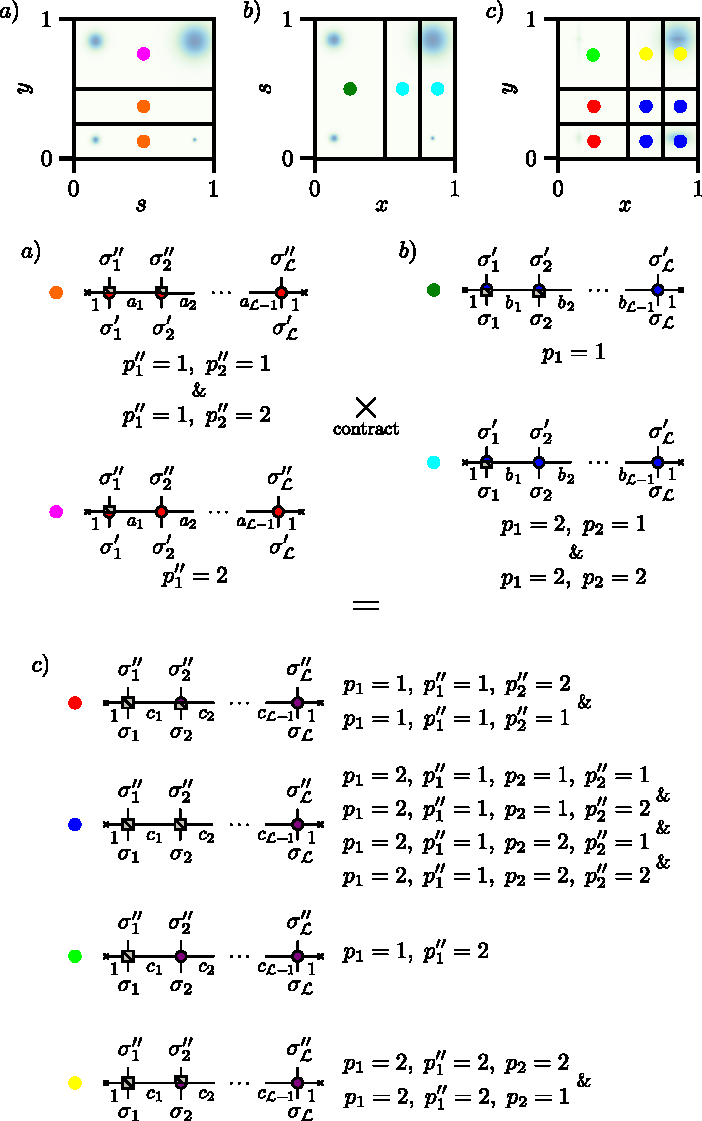
\includegraphics{figures/2DPatchContrRepr.pdf}
    \caption{2D representation of patched MPO-MPO contraction.}
    \label{fig:2DPatchContrRepr}
\end{figure}

\prettyref{fig:2DPatchContrRepr} illustrates the idea for two well-constructed collections of patched MPOs, \(A\) and \(B\).  
Each MPO patch is first unfolded into an MPS and mapped to its assigned region of the two–dimensional domain, exactly as described in the preceding chapter for pQTCI.  
Panels~$(a)$ and~$(b)$ show the resulting patch ensembles for \(A\) and \(B\), respectively.  
Every \(A\)-patch is then paired with every \emph{compatible} \(B\)-patch and contracted over their shared indices \(\boldsymbol{\sigma}'\) ($s$ variable), covering all index combinations permitted by the internal projections\footnotemark.
\footnotetext{In the particular example of \prettyref{fig:2DPatchContrRepr} no constraints due to internal indices' projections are imposed. Hence, every $A$-patch is contracted with every $B$-patch.}  
The collection of contraction results tiles the square
\([0,1]^{2}\), furnishing a patched representation of the product tensor~\(C\).

As highlighted by the first row of \prettyref{fig:2DPatchContrRepr}, this patchwise contraction behaves as a ``matrix multiplication'' of patches:  
\begin{itemize}
    \item the patching depth along the \emph{columns} (\(x\)-direction) of the final
  object is inherited from the row patching of the left factor \(A\);  
  \item the patching depth along the \emph{rows} (\(y\)-direction) is inherited
  from the column patching of the right factor \(B\).
\end{itemize}
Although the schematic in \prettyref{fig:2DPatchContrRepr} employs a simple, regular subdivision to convey the basic logic of \emph{patched contractions}, real applications involve far more intricate patch patterns and additional constraints on the internal indices, making the general contraction problem correspondingly richer and more challenging.

The diagrammatic picture introduced in \prettyref{fig:2DPatchContrRepr} is not restricted to MPOs that come
from a two–dimensional, interleaved quantics TT unfolding.  
It extends naturally to higher physical dimensions.  
Suppose that we have a set of $\mR$ indices each of dimension $d$, then we can assign to it real variable $x$ discretised in base~\(d\) such as
\begin{equation}
  x \;\mapsto\; x(\boldsymbol{\sigma})
  \;=\;
  \sum_{r=1}^{\mathcal R}\sigma_{r}\,d^{-r},
  \qquad
  \sigma_{r}\in\{1,\dots,d\}.
\end{equation}
The corresponding axis will then be partitioned into \(d\) intervals at each digit (rather than two), and the same two–dimensional patch contraction picture can be drawn.  
In fact, the internal indices \(\boldsymbol{\sigma}'\) and the external indices \(\boldsymbol{\sigma}\), \(\boldsymbol{\sigma}''\) may even carry different local dimensions $d, d'$ and $d''$. Provided that the internal local dimensions are equal for the two factors, i.e. $\text{dim}(\sigma_\ell^{\prime A}) =
\text{dim}(\sigma_\ell^{\prime B})$ $\forall \ell$, the two–dimensional representation retains its generality.

This grid view is especially convenient when modelling convolution–type integrals—\emph{i.e.}, “matrix multiplications” of two-dimensional functions—such as
\begin{equation}
  h(x,y)
  \;=\;
  \int_{0}^{1}\!ds\;f(x,s)\,g(s,y).
\end{equation}
Here each patch pair encodes the actual contribution of a specific \((x\!\times\!s)\!\otimes\!(s\!\times\!y)\) block to the result \(h(x,y)\), and the patched contraction tiles the \([0,1]^{2}\) domain exactly. 

The foregoing analysis suggests that coupling pQTCI with a patch-wise contraction scheme can dramatically curb the computational expense of many tensor-network tasks—particularly when the underlying functions are highly
localised.  Before presenting concrete benchmarks for this combined approach, we first examine the expected cost reductions and performance benefits of patch-level contractions across several representative classes of MPO–MPO products.

\subsection{Patched element-wise multiplication}
Let $\widetilde{A}_{\bsigma}$ and $\widetilde{B}_{\bsigma}$ be two MPSs.  We seek their \textit{Hadamard (element-wise) product} \cite{Lee2018}
\begin{equation}
    C_{\bsigma} = A_{\bsigma}\,\raisebox{.5pt}{\textcircled{\raisebox{-3pt}{*}}}\,B_{\bsigma}
\end{equation}
meaning that every entry of $C$ is obtained by multiplying the corresponding entries of $A$ and $B$; $C_{\bsigma} = A_{\bsigma}B_{\bsigma}$ for all index tuples $\bsigma$. 
To carry out the element-wise product with TTs we first need to embed each tensor train unfolding of the factors in a \emph{diagonal} MPO:
\begin{equation}
    \begin{aligned}
      \widetilde{B}_{\bsigma} &= \raisebox{-7mm}{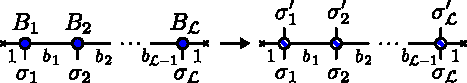
\includegraphics{figures/BDiagMPO.pdf}} := \widetilde{B}^D_{\bsigma\bsigma'}\\
       \widetilde{A}_{\bsigma} &= \raisebox{-7mm}{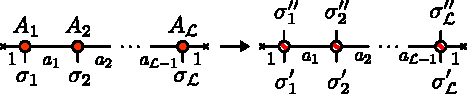
\includegraphics{figures/ADiagMPO.pdf}} := \widetilde{A}^D_{\bsigma'\bsigma''}
    \end{aligned}
    \label{eq:diagMPOs}
\end{equation}

where each local tensor is defined by

\begin{equation}
    \label{eq:diagSiteTensors}
    \begin{aligned}
        \raisebox{-6mm}{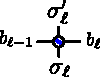
\includegraphics{figures/BDiag_SiteTensor.pdf}} = \begin{cases}
            [B^{\sigma_\ell}_\ell]_{b_{\ell-1},b_\ell} \quad &\text{if}\ \sigma'_\ell = \sigma''_\ell \\
            [0]_{b_{\ell-1},b_\ell} \quad &\text{otherwise}.
        \end{cases}\\
        \raisebox{-6mm}{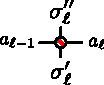
\includegraphics{figures/ADiag_SiteTensor.pdf}} = \begin{cases}
            [A^{\sigma'_\ell}_\ell]_{a_{\ell-1},a_\ell} \quad &\text{if}\ \sigma_\ell = \sigma'_\ell \\
            [0]_{a_{\ell-1},a_\ell} \quad &\text{otherwise}
        \end{cases}
    \end{aligned}
\end{equation}
The site indices of the original TTs have been relabelled to make the subsequent contraction explicit:
\begin{equation}
    \raisebox{-0.8cm}{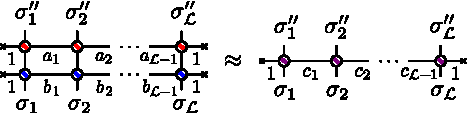
\includegraphics{figures/DiagMPOMPOcontr.pdf}}.
    \label{eq:diagMPOcontr}
\end{equation}
From this contraction we read off the resulting tensor-train
\begin{equation}
    \widetilde{C}_{\sigma} = \raisebox{-5.5mm}{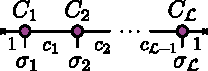
\includegraphics{figures/CTensorTrain.pdf}} \quad \text{with} \quad \raisebox{-6.5mm}{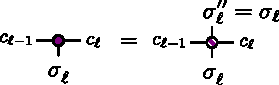
\includegraphics{figures/UnDiag_SiteTensor.pdf}}.
\end{equation}
Hence $\widetilde{C}$ represents the Hadamard product
$C_{\boldsymbol{\sigma}}=A_{\boldsymbol{\sigma}}B_{\boldsymbol{\sigma}}$ in TT form. The MPO-MPO contraction in \prettyref{eq:diagMPOcontr} can be performed using the standard MPS-toolkit \cite{ITensors.jl, QSpace}, however if we apply the patching scheme upon the factor tensors $A$ and $B$, the patched contraction routine can be employed.

\prettyref{eq:diagSiteTensors} shows that a \emph{diagonalised} MPO can sensibly be patched only along \emph{identical} input and output indices, because each site tensor is non–zero solely when \(\sigma''_{\ell}=\sigma'_{\ell}\) (or, equivalently, when \(\sigma'_{\ell}=\sigma_{\ell}\)).
Hence, it is unnecessary to unfold the diagonal MPOs of \prettyref{eq:diagMPOs} and \prettyref{eq:diagMPOcontr} into yet another MPS representation.  
Instead, we may work directly with the original MPS forms
\(\widetilde{A}_{\boldsymbol{\sigma}}\) and
\(\widetilde{B}_{\boldsymbol{\sigma}}\) and apply the patching routine to them.  Only those patches whose domains \emph{overlap} will yield a non–vanishing contraction, making the two–dimensional patch diagram
introduced earlier particularly transparent in this setting. We now illustrate the idea with a concrete example.

Consider two tensor trains \(\widetilde{A}_{\boldsymbol{\sigma}}\) and \(\widetilde{B}_{\boldsymbol{\sigma}}\) that represent two-dimensional functions on the unit square, both obtained via the pQTCI routine.  
As before we map the interleaved index string
\(\boldsymbol{\sigma}=(\sigma_{1},\sigma_{2},\dots \sigma_{2\mR})\) to the auxiliary variables
\begin{equation}
    x \mapsto \sum_{r=1}^{\mR}\sigma_{2r-1}2^{-r}, \quad y \mapsto \sum_{r=1}^{\mR}\sigma_{2r}2^{-r}, \quad \sigma_{2r}, \sigma_{2r-1} \in \{0,1\}
\end{equation}
so that each patch corresponds to a tile in the \([0,1]^{2}\) domain.  
Because we perform an \emph{element-wise} (Hadamard) product, the two operands share the same \((x,y)\)  grid; only patches whose tiles overlap contribute to
the result, as sketched in \prettyref{fig:patchElemContr}. 
\begin{figure}
    \centering    
    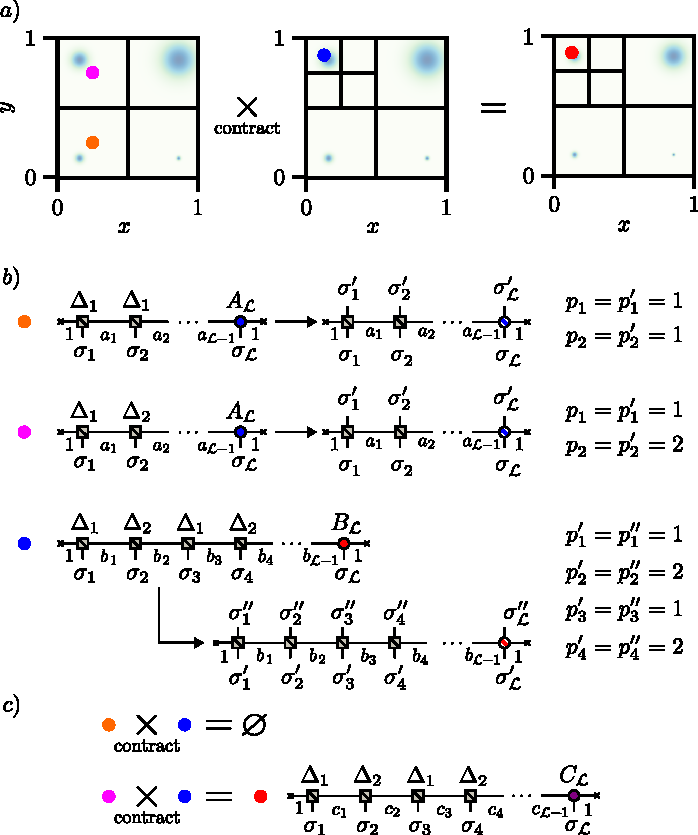
\includegraphics{figures/PatchElemenContr.pdf}
    \caption{Patched element-wise contraction. $(a)$  Two–dimensional domain tiled by patches visualised via the auxiliary variables
    \(x(\sigma_{1},\sigma_{3},\dots)\) and
    \(y(\sigma_{2},\sigma_{4},\dots)\). $(b)$  Representative patches in tensor form: each patch is shown first in the TT format as produced by pQTCI and then in its diagonalised MPO version obtained with \prettyref{eq:diagSiteTensors}. $(c)$  Patchwise multiplication for the patches marked by coloured dots; only those whose tiles overlap in the domain yield non-zero results. } 
    \label{fig:patchElemContr}
\end{figure}

Assume that both \(A\) and \(B\) are decomposed into the same number of patches, \(\Np\), and that every patch has a capped bond dimension \(\chip\).  
The patched routine executes approximately
\(\Np \) MPO–MPO contractions.  
Employing the zip-up algorithm (or an equivalent
\(\mathcal{O}(\chi^{4}d^{4}\mathcal L)\) scheme) for each local contraction, the total arithmetic cost of element-wise MPS multiplication scales as

\begin{equation}
    \order(\Np\chip^4d^4\mL). 
\end{equation}

To outperform a single, non-patched contraction of the full-rank MPOs (\(\chi\) being their common bond dimension), the number of patches must obey 

\begin{equation}
    \Np < \frac{\chi^4}{\chip^{\,4}}.
    \label{eq:elemMulBound}
\end{equation}

Within this window patch-wise element-wise multiplication delivers a net computational saving by trading rank for patch count.


\subsection{Patched matrix multiplication}

Let \(\widetilde{L}_{\boldsymbol{\sigma}}\) and \(\widetilde{R}_{\boldsymbol{\sigma}}\) be two generic matrix-product states (MPS).  The first carries index sets \(\boldsymbol{\sigma}^{R},\boldsymbol{\sigma}^{S}\), the second \(\boldsymbol{\sigma}^{S},\boldsymbol{\sigma}^{C}\).  
Using the mapping of Eq.~\eqref{eq:MPStoMPO}, each MPS can be reshaped into an MPO:
\begin{align}
        \nonumber\widetilde{R}_{\bsigma} &= \raisebox{-7mm}{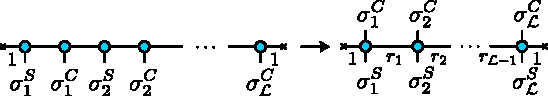
\includegraphics{figures/RightMPO.pdf}} := \widetilde{R}_{\bsigma^S\bsigma^C}\\
        {}\\
        \nonumber\widetilde{L}_{\bsigma} &= \raisebox{-7mm}{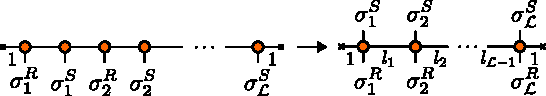
\includegraphics{figures/LeftMPO.pdf}} := \widetilde{L}_{\bsigma^R\bsigma^S}
        \label{eq:matMulMPOs}
\end{align}
    


Here each composite index (e.g.\ \(\sigma^{R}_{\ell}\)) can represent a single index or a block of neighbouring
physical indices of a parent MPS and every correspondent MPS core is obtained by contracting the corresponding block of neighbouring MPS site tensors.

With this interpretation, the standard MPO-MPO contraction between $\widetilde{L}$ and $\widetilde{R}$
\begin{equation}
    \label{eq:matMulConntr}
    \widetilde{M}_{\bsigma^R\bsigma^C} = \sum_{\bsigma^S} \widetilde{L}_{\bsigma^R\bsigma^S}\widetilde{R}_{\bsigma^S\bsigma^C} = \raisebox{-10mm}{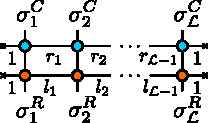
\includegraphics{figures/MatMulMPOContr.pdf}}
\end{equation}
acts exactly like a \emph{matrix multiplication} between two tensor-train–style objects, producing an MPO indexed by
\(\boldsymbol{\sigma}^{R}\) and \(\boldsymbol{\sigma}^{C}\). The labeling becomes then much clearer: $\bsigma^R$, $\bsigma^C$ and $\bsigma^S$ represent the row, column and shared indices of our ``matrices'' $L$ and $R$.

Assume that \(L_{\bsigma^{R}\bsigma^{S}}\) and \(R_{\bsigma^{S},\bsigma^{C}}\) are pQTCI
approximations of two multivariate functions,

\begin{equation}
    L(\boldsymbol{x}(\bsigma^R), \boldsymbol{s}(\bsigma^S)) = L_{\bsigma^R, \bsigma^S}, \quad  R(\boldsymbol{s}(\bsigma^S), \boldsymbol{y}(\bsigma^C)) = R_{\bsigma^S, \bsigma^R}
\end{equation}

respectively, their contraction realises the convolution 
\begin{equation}
    M(\boldsymbol{x},\boldsymbol{y}) =\int d\boldsymbol{s} L(\boldsymbol{x}, \boldsymbol{s})R(\boldsymbol{s}, \boldsymbol{y}).
    \label{eq:convTypeInt}
\end{equation}


\begin{figure}[ht!]
\centering
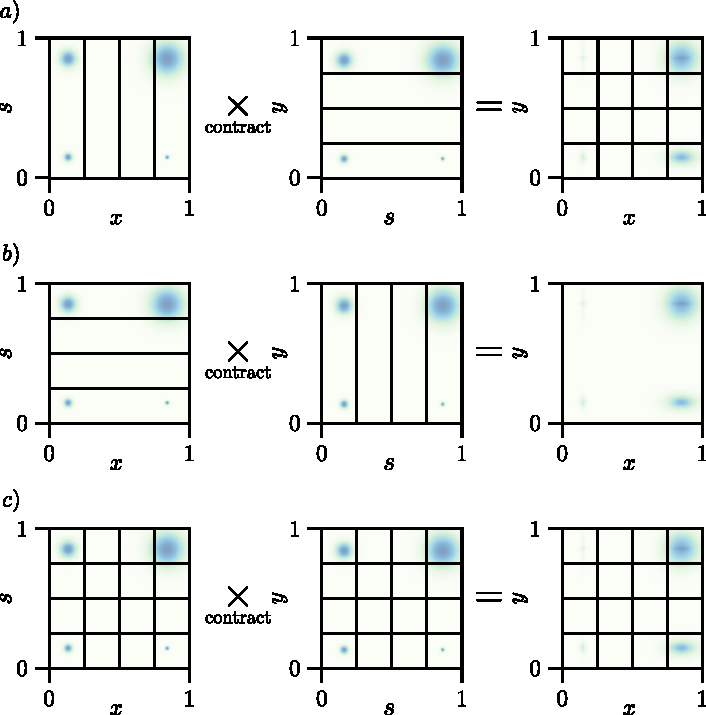
\includegraphics{figures/2DPatchMatMul.pdf}
\caption{Patched \textit{matrix multiplication}. $(a)$ Worst-case scenario. Each patch in the first factor is contracted with \textit{each} patch in the second factor. $(b)$ Best-case scenario. Each patch in the first factor is contacted with a \textit{single} patch in the second factor. $(c)$ Average case scenario. Each patch in the first factor is contracted with a \textit{limited set} of patches in the second factor.}
\label{fig:2DPatchMatMul}
\end{figure}

\prettyref{fig:2DPatchMatMul} visualises three patching patterns for this “MPO–matrix multiplication,” assuming each factor is decomposed into \(\Np \) patches of equal bond dimension \(\chip\). There the first column corresponds to the $L$ patched tensor, the second column to the $R$ and the last column of panels to the patched contraction result $M$. The possible scenarios are the following:

\begingroup
\renewcommand{\labelenumi}{(\alph{enumi})}
\begin{enumerate}
\item \textbf{Worst case} (first row):  
      only the external indices are patched, so every \(L\)-patch contracts
      with \emph{every} \(R\)-patch.  
      The \(\Np^{2}\) contractions cost
      \begin{equation}
        \label{eq:worsScaling}
        \mathcal{O}\bigl(
           \Np^{2}\,
           \chip^{\,4}\,d^{4}\,\mathcal L
        \bigr),
      \end{equation}
      improving on a full-rank contraction iff
      \begin{equation}
       \Np<\frac{\chi^{2}}{\chip^{2}}.
       \label{eq:worstBound}
      \end{equation}
      

\item \textbf{Best case} (centre row):  
      the shared index \(\boldsymbol{\sigma}^{S}\) is patched so that each
      \(L\)-patch matches exactly one \(R\)-patch.  
      The \(\Np \) contraction cost scale as
      \begin{equation}
        \mathcal{O}\bigl(
          \Np \,
          \chip^{\,4}\,d^{4}\,\mathcal L
        \bigr),
      \end{equation}
      yielding a gain whenever
      \begin{equation}
       \Np<\frac{\chi^{4}}{\chip^{4}}.
       \label{eq:bestBound}
      \end{equation}

\item \textbf{Average case} (bottom row):  
      both external and shared indices are patched.  
      After \(\bar\ell\) subdivision steps on a uniform \(d\)-ary grid the
      number of admissible patch pairs is
      \(d^{\bar\ell}\,d^{\bar\ell( D-1)/D}
       =\Np^{(2D-1)/D}\), where $d^{\ellb}= \Np$ for a uniform grid and $D=\mN$ for the interleaved ordering (\textit{i.e.} the dimensionality of the functions $L(x_1,\dots,x_{\mN/2},s_1,\dots,s_{\mN/2})$ and $R(s_1,\dots,s_{\mN/2},y_1,\dots,y_{\mN/2})$) and \(D=2\) for fused.
      The overall cost becomes
      \begin{equation}
        \mathcal{O}\bigl(
          \Np^{\frac{2D-1}{D}}\,
          \chip^{\,4}\,\mathcal L
        \bigr),
      \end{equation}
      advantageous as long as
      \begin{equation}
        \Np<\left(\frac{\chi}{\chip}\right)^{\frac{4D}{2D-1}}.
        \label{eq:averageBound}
      \end{equation}
\end{enumerate}
\endgroup

Patch-wise matrix multiplication trades global bond dimension for patch count.  When any of the bounds in \prettyref{eq:bestBound}, \prettyref{eq:worstBound} and \prettyref{eq:averageBound} are respected, patched MPO–MPO contractions has the possibility\footnotemark\, to outperform their monolithic counterparts, making them a compelling tool for high-dimensional convolutions.
\footnotetext{The typical result out of a pQTCI run is a combination of the patterns shown in \prettyref{fig:2DPatchMatMul}, due to the adaptivity of the algorithm. Hence, \prettyref{eq:bestBound}, \prettyref{eq:worstBound} and \prettyref{eq:averageBound} only give us an intuition of the optimal bounds for $\Np$.}
\section{Adaptive Patched MPO-MPO Contraction}
\label{sec:AdaptivePatchMPOMPOContr}

Building on the principles of pQTCI, we now propose an \emph{adaptive} contraction scheme that further curbs the memory and runtime requirements of
patched MPO–MPO products.  
The primary bottleneck in any contraction routine is the peak \textsc{ram} footprint, which grows steeply with the bond dimension of the tensors being multiplied.  By dynamically refining the factor MPOs whenever their local bond dimension exceeds a prescribed cap, we can keep the intermediate contraction costs in check. The resulting procedure, which we term the \emph{adaptive patched MPO–MPO contraction} (or \emph{adaptive Matrix Multiplication}), combines patched contractions with a bond–dimension–driven refinement loop, similar to pQTCI.

\subsection{MPO slicing}
The key technical ingredient is an MPO analogue of the MPS \emph{slicing} operation (cf.\ \prettyref{eq:tensorSlice}).  Because every MPO can be unfolded into an MPS (see \prettyref{eq:resultPatchContr} and \prettyref{eq:resultMPSPatchContr}), we may

\begingroup
\renewcommand{\labelenumi}{(\roman{enumi})}
\begin{enumerate}
  \item unfold the operator to an MPS,
  \item project the state onto a subtensor specified by a prefix, \textit{e.g.} \((p_{1},p_{2},\dots,p_{\ellb})\), and
  \item fold the sliced MPS back into an MPO via
     \prettyref{eq:patchMPStoMPO}.
\end{enumerate}
\endgroup

\prettyref{fig:MPOSlicing} illustrates this “MPO slicing’’ workflow.

\begin{figure}[ht!]
    \centering
    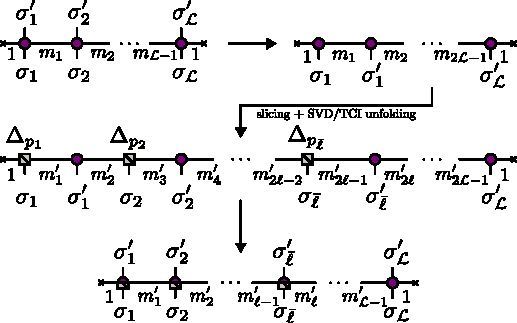
\includegraphics{figures/SlicingMPO.pdf}
    \caption{Slicing of an MPO}
    \label{fig:MPOSlicing}
\end{figure}
The slicing procedure illustrated in \prettyref{fig:MPOSlicing} lets our algorithm reuse the TT-projection routines of pQTCI for MPOs. In addition, retaining each patch as an MPS instead simplifies site-tensor manipulation and index bookkeeping; each patched MPS is converted into an MPO only immediately before a contraction step.

\subsection{The algorithm}
Given two MPOs \(\widetilde{A}_{\bsigma\bsigma'}\) and \(\widetilde{B}_{\bsigma'\bsigma''}\) (cf. \prettyref{eq:2MPOs}), the adaptive patched contraction attempts to compute the ``matrix multiplication'':
\begin{equation}
    \widetilde{C}_{\bsigma'\bsigma''} = \sum_{\bsigma'} \widetilde{A}_{\bsigma\bsigma'} \widetilde{B}_{\bsigma'\bsigma''}
    \label{eq:genericAdaptiveMPOMPOContr}
\end{equation}
as follows
\begingroup
\renewcommand{\labelenumi}{(\arabic{enumi})}
\begin{enumerate}
    \item
  Fix a bond–dimension cap \(\chip\) and a target accuracy \(\tau\).  
  Attempt a \emph{single} MPO–MPO contraction.  
  If the product \(\widetilde{C}_{\bsigma\bsigma''}\) converges to tolerance with rank \(\chi<\chip\), terminate.
\item Otherwise, slice both MPOs along their first external physical indices,
  producing
  \begin{equation}
    \widetilde{A}_{\bsigma,\bsigma'}^{\,p_{1}},
    \quad
    \widetilde{B}_{\bsigma',\bsigma''}^{\,p''_{1}},
    \qquad
    p''_{1}\in\{1,\dots,d''_{1}\},
    \;
    p_{1}\in\{1,\dots,d_{1}\},
  \end{equation}
  via the MPO–slicing routine of \prettyref{fig:MPOSlicing}.
    \item Contract every \emph{compatible} pair \(\bigl(\widetilde{A}^{\,p_{1}},
          \widetilde{B}^{\,p''_{1}}\bigr)\),
  enforcing the bond cap \(\chip\) on each local product.
\item For each partial product
  \(\widetilde{C}^{\,p_{1},p''_{1}}\) that still fails to converge (\texttt{tasks}), slice it further along the \(\bsigma\) and \(\bsigma''\) axes while storing any converged patch (\texttt{results}).
\item Repeat steps~$(3)$–$(4)$, recursively increasing the slicing depth, until no unconverged patched MPOs remain.
\end{enumerate}
\endgroup

\begin{figure}[ht!]
    \centering
    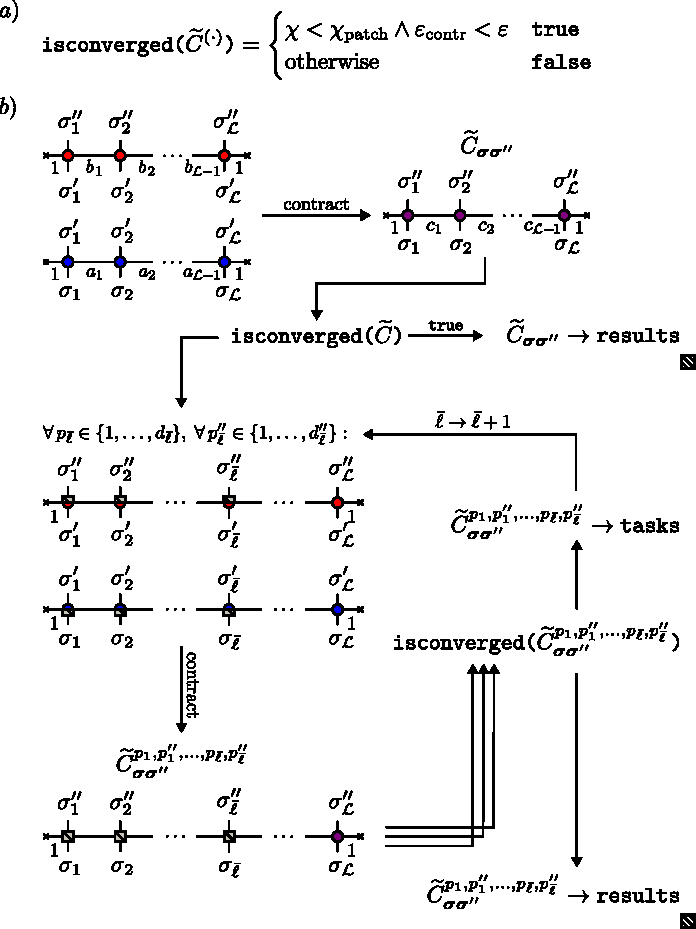
\includegraphics{figures/AdaptivePatchContr.pdf}
    \caption{Adaptive patched MPO–MPO contraction. $(a)$ Convergence test for a patch
    \(\widetilde{C}^{\,p_1,p''_1,\dots,p_{\bar\ell},p''_{\bar\ell}}\), governed by the bond–dimension cap \(\chip\) and the accuracy tolerance \(\tau\). $\varepsilon_{\text{contr}}$ represents the error of the contraction result. $(b)$ Flowchart of the algorithm.
    The global MPO product is recursively broken into smaller sub-problems via \emph{MPO slicing}
    (\prettyref{fig:MPOSlicing}).
    Each subtensor pair is contracted under the bond cap $\chip$; converged patches are moved to \texttt{results}, while the remaining ones are
    placed back into \texttt{tasks}.
    The routine halts -- \raisebox{-0.2ex}{
\includegraphics[scale=0.95]{figures/TerminalSquare.pdf}} -- once \texttt{tasks} is empty. See the text for a step-by-step description.}
    \label{fig:adaptiveMatMul}
\end{figure}

A few remarks are in order. At first sight the adaptive routine might seem more expensive than a single MPO--MPO contraction.  In practice this overhead is negligible: for a fixed tolerance~$\tau$ each local contraction is \emph{aborted} as soon as its bond dimension hits the cap~$\chip$ (e.g.\ by truncating 
the SVD step at the desired cutoff in the zip--up sweep, \prettyref{fig:zipupalg}). Although up to
\(\mathcal{O} \bigl(d^{\bar\ell}(d'')^{\bar\ell}\bigr)\) patched MPO pairs may be
processed---\(\bar\ell\) being the deepest slicing level of the MPS unfolded factors $\widetilde{A}$ and $\widetilde{B}$---each individual multiply is cheap thanks to the tight rank bound $\chip$.

The second remark concerns the choice of patching indices. Our implementation slices only the \emph{external} index sets \(\bsigma\) and \(\bsigma''\); consequently the total number of multiplications is \(N=\Np^{2}\), matching the worst--case scaling in \prettyref{eq:worsScaling}.  This choice is,
however, deliberate:  
\begingroup
\renewcommand{\labelenumi}{(\alph{enumi})}
\begin{enumerate}
  \item the arithmetic cost remains
        \(\mathcal{O} \bigl(N\,\chip^{4}\,d^{4}\,\mL \bigr)\), so memory is still controlled by~\(\chip\), which is fixed and therefore independent of the particular slicing choice;
  \item the refinement is in this way \emph{feature--adaptive}: whenever a patch  \(\widetilde{C}^{p_1,p''_1,\dots}\) fails to converge (its local rank exceeds \(\chip\)) the algorithm subdivides exactly that output configuration space $(\bsigma, \bsigma'')$ region, yielding a finer discretisation where the product tensor \(\widetilde{C}_{\bsigma \bsigma''}\) is most intricate. Slicing the internal indices \(\bsigma'\) instead of the external ones would also reduce the contraction cost by capping the bond dimension at $\chip$, but at the expense of this adaptive focus.
\end{enumerate}
\endgroup

The \emph{adaptive patched MPO--MPO contraction} shown in \prettyref{fig:adaptiveMatMul} bounds the local bond dimension to limit memory usage while simultaneously producing a patch decomposition that concentrates effort where the result is most complex, thus delivering the same kind of problem--tailored efficiency achieved by pQTCI.



